%
We will here investigate how our results scales with $B$.
In \cref{chap:linear} we saw how the linear growth rates depends on $B$, and we would to further investigate the $B$-dependency of the system by comparing the profiles in the steady state for various $B$ and by comparing the results from the saturated turbulent phase.

This is motivated by the experimental findings in linear machines, where one has observed a gradual onset of the turbulence with more and more modes interacting with an increasing $B$-field \cite{Klinger1997,Klinger1997a,Burin2005}.
The onset in form of singular modes has not been observed in the simulations.
Instead, a threshold $B_0$ is found for the onset of turbulence (see \cref{fig:grB}).
Therefore, only $B_0 = 0.06\T \to 0.1\T$ reaches the saturated turbulent state in the simulations.
The simulations with $B_0 = 0.02\T$ is stable against the perturbation, and the simulations with $B_0 = 0.04\T$ has a very slow growth rate%
\footnote{It is expected that $B_0=0.04\T$ eventually will reach the saturated turbulent state as the growth rate is positive.
    However, as the maximum growth rate of $B_0=0.04\T$ is about one tenth of the maximum growth rate of $B_0=0.06\T$, the simulations would be need to be run approximately ten times longer in order to reach the saturated turbulent state.
}
%
.
This is in qualitative agreement with what is observed in \cite{Burin2005}.

Finally, note that the normalizing $B$ in \cref{eq:celma_vortD,eq:celma_dens,eq:celma_mom_dens,eq:celma_j_par,eq:celma_vortD_evolution} can always be chosen to be $1$.
However, $B$ appears in the set of equations through $\om_{ci}$, which means that it effectively sets the time step (in real variables) through $\breve{t}=t\om_{ci}^{-1}$.
This in turn affects the $\rho_s$ (as $\rho_s=c_s/\om_{ci}$), and thus the normalized domain size.

\section{The steady state profiles}
\label{sec:BScanSS}
%
\Cref{fig:BScanPar} shows the parallel profile variations as a function of $B_0$.
%
\begin{figure}[htb]
    \centering
    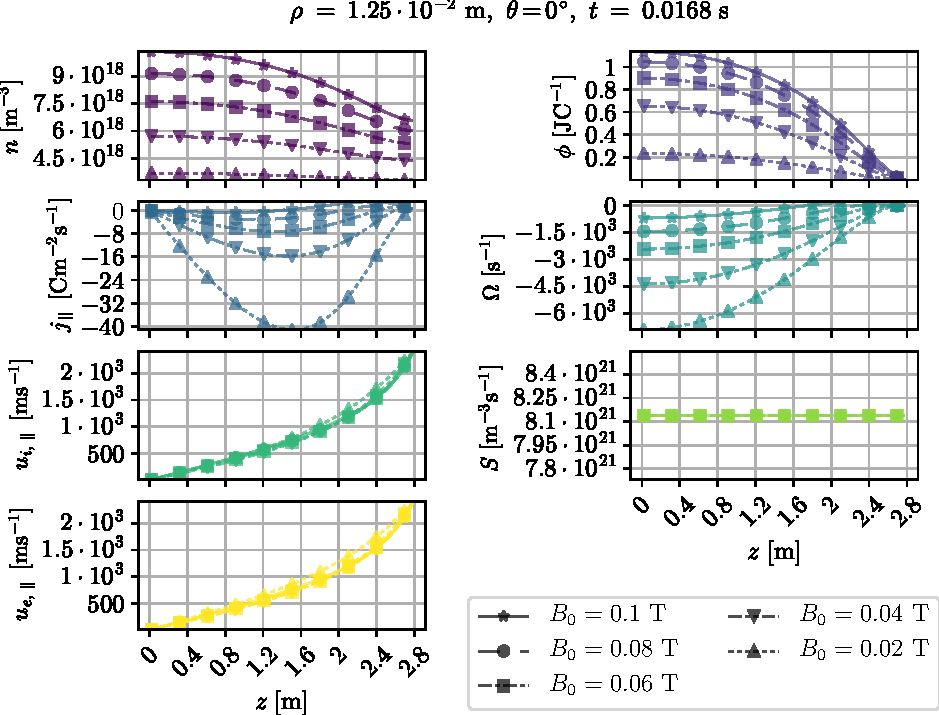
\includegraphics{fig/results/bScan/BScanPar}
    \caption{The parallel steady state profiles as a function of $B_0$.}
    \label{fig:BScanPar}
\end{figure}
%
We note that $n$ is increasing with increasing $B$-field.
This can be explained by the increase in parallel velocities, which will be further explained in the discussion of the radial profiles.
Although $j_\| \propto n$, we can observe that the absolute magnitude decreases with increasing $B$, signifying that the parallel electron and ion velocities are closer to each other.
As a consequence, the parallel derivatives of $j_\|$ decreases, which in turn means that the absolute amplitude of the vorticity decreases.
$\phi$ retains a Boltzmann-like distribution for all $B$-fields, which means that $\phi$ must decrease in the parallel direction as $n$ decreases.

%
\begin{figure}[htb]
    \centering
    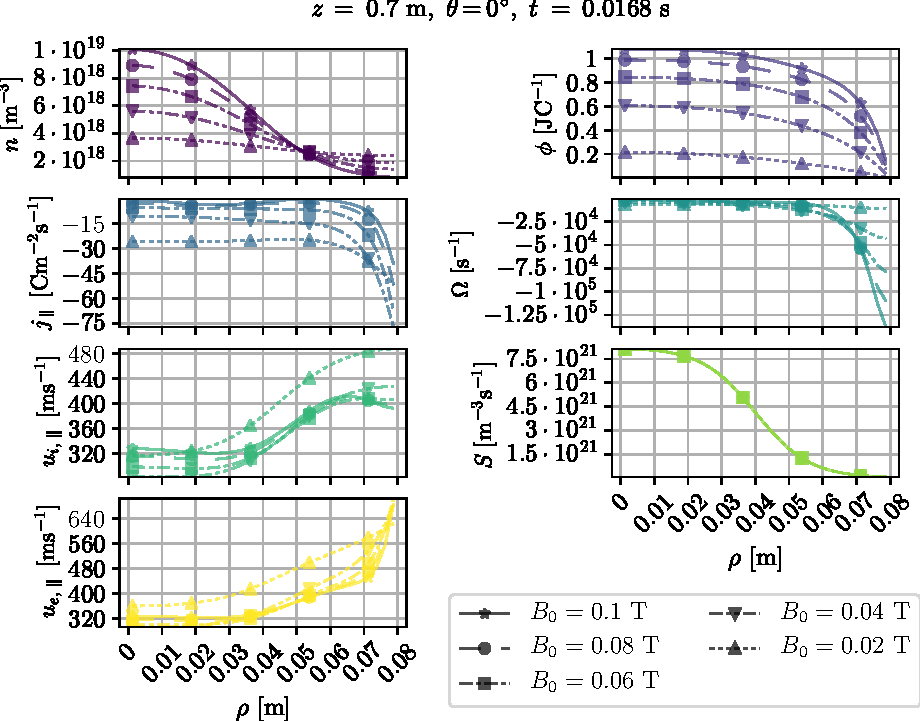
\includegraphics{fig/results/bScan/BScanRad}
    \caption{The radial steady state profiles as a function of $B_0$.}
    \label{fig:BScanRad}
\end{figure}
%
As indicated in the radial direction in \cref{fig:BScanRad}, $\phi$ is increasing with increasing $B$-field due to the Boltzmann-like distribution for each parallel position.
Since the potential is fixed to $0$ at $\rho = L_\rho$, we must have that the gradients gets sharper for increasing $B$-fields.
This has the consequence that the vorticity gets higher for increasing $B$.

From this, we will give an explanation for the observed increase in $n$ for increasing $B$ here.
As mentioned in \cref{sec:fluxes}, almost no plasma can leave the domain in the perpendicular direction due to the boundary condition $\L.\phi\R|_{L_\rho}=0$ and shallow parallel second derivatives.
Hence, we must mechanisms in which the plasma can leave the domain in the parallel direction.
We note that the in the parallel momentum equation, the right hand sides equals to first order $-T_i \grad_\| n + n_\a q_\a \grad_\| \phi$.
As the parallel gradients increases for increasing $B$ field, the pressure cannot account for the increased parallel outflux.
On the other hand, the potential term can account for at least part of the increased parallel outflux.
As the sign of this term depends on the species types, there will be less difference in this term for lower values of $B$, and since the system seeks a steady state the ions will slow the electron flux less.
However, as the decrease in $\grad_\| \phi$ comes from the decrease in $n$ with decreasing $B$, it cannot account for the initial depletion of density for decreasing $B$.
Is it possible that this initial depletion can come from the fact that the systems searches for balance between the parallel currents and $\Omega$ in order to reach the steady state, and that the higher radial boundary value at $\Omega$ must be balanced by higher parallel velocities.

$n\propto B$ is also observed in helicon experiments, as stated by for example \cite{Tynan2006a}.
However, this trend in the experiments is more likely due to the coupling between the helicon wave and resonances in the plasma.
Of course, higher confinement due to smaller Larmor radii is also contributing to this, but the contribution is believed to be small as the plasma is lost at a higher rate in the parallel direction than in the radial direction due to high parallel velocities.

Finally, it is worth nothing that the artificial viscosity is kept constant in the normalized equations.
This means that they will increase for decreasing $B$, as they are normalized with $\om_{ci}$.
However, they are small compared with the other terms, and can therefore not account for the trend in $n$ when the magnetic field strength changes.

\section{Variations in turbulence}
%
From what we discussed in \cref{sec:BScanSS}, it is intuitive to expect that the turbulence levels increases with increasing $B$ as the gradients gets steeper, and can therefore act as a bigger source of energy to the turbulent fluctuations.
That the turbulent amplitude is decreasing can be seen from the standard deviation of the time average of the poloidal average of $n$ in \cref{fig:BScanPosOfFluct}.
%
\begin{figure}[htb]
    \centering
    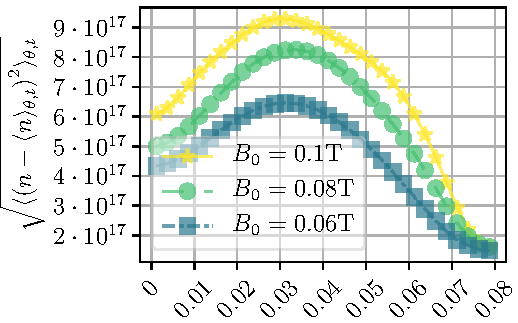
\includegraphics{fig/results/bScan/BScanPosOfFluct}
    \caption{The standard deviation for the turbulent cases.}
    \label{fig:BScanPosOfFluct}
\end{figure}
%

The position of the maximum fluctuation amplitude stays the same, whereas the maximum itself decreases for decreasing $B$.
The same behavior is found in the potential fluctuations.
Consequently, the density profiles are flattened for all $B$, but decreasing with decreasing $B$ due to the lower amplitude of the fluctuations.

We can also investigate how the skewness and kurtosis is changing when varying $B$, by inspecting \cref{fig:BScanSkewKurt}.
%
\begin{figure}[htb]
    \centering
    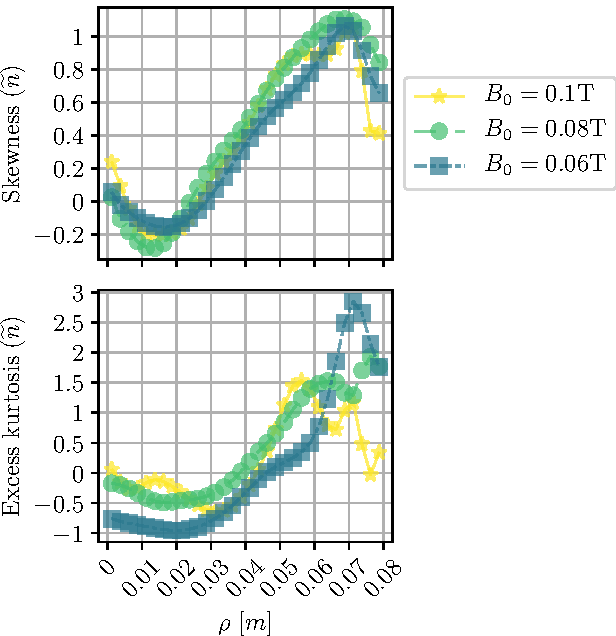
\includegraphics{fig/results/bScan/BScanSkewKurt}
    \caption{The skewness and kurtosis for the turbulent cases.}
    \label{fig:BScanSkewKurt}
\end{figure}
%
Note that these parameters does not say anything about the amplitude of the perturbation, but rather how the probability of perturbations are distributed.
We can observe that although the amplitude of the perturbations are changing, the distribution stays roughly the same, with exception of the edge of the cylinder, where the there is a higher chance for extreme events in the case of $B=0.06\T$.
This does not necessarily mean that more "blobs" or "holes" are found, as the triggering signal is set for the radial flux.

The blob and hole count per time as a function of the magnetic field is given in \cref{fig:BScanBlobCount}.
%
\begin{figure}[htb]
    \centering
    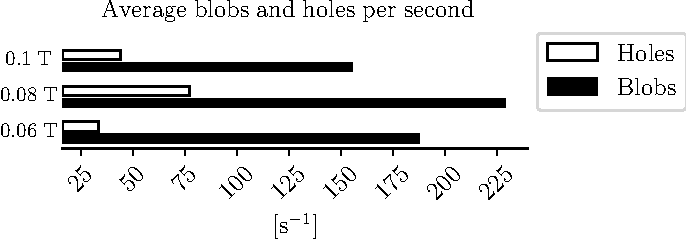
\includegraphics{fig/results/bScan/BScanBlobCount}
    \caption{The blob count as a function of $B_0$ for a triggering signal of $3\sigma$ on the radial flux.}
    \label{fig:BScanBlobCount}
\end{figure}
%
One be careful to say anything conclusive about this as very few events was found, as shown in \cref{tb:blobAndHolesCount}, but the decrease of the blob and holes count could be account for by the strong poloidal shear seen from the vorticity in \cref{fig:BScanPar}.
%
\begin{center}
        \colorme
        \begin{tabular}{l|cc}
            \hline
            Field strength in $[\T]$ & Blobs count & Holes count\\
            \hline
            $0.06$ & $19$ & $2$ \\
            $0.08$ & $14$ & $4$ \\
            $0.10$ & $ 2$ & $1$ \\
            \hline\hline
        \end{tabular}
        \label{tb:blobAndHolesCount}
\end{center}
%

Finally, in this section, we will address how the flux is scaling with the magnetic field strength.
%
\begin{figure}[htb]
    \centering
    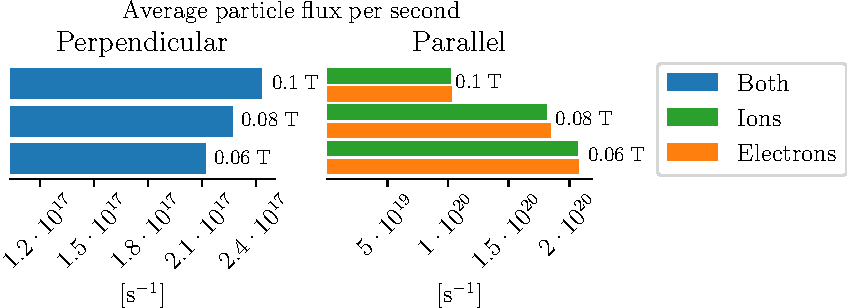
\includegraphics{fig/results/bScan/BScanTotalFlux}
    \caption{
        The variation of the total flux as a function of $B_0$.
        The point of measurement is the same as in \cref{fig:flux008}.
    }
    \label{fig:BScanTotalFlux}
\end{figure}
%
\Cref{fig:BScanTotalFlux} shows the trend.
As discussed above, the increased electron and ion velocities will give rise to a higher radial flux.
Hence, we observe a decrease in the parallel flux for higher $B$.
The converse is true for the perpendicular flux.
This is consistent with what was observed in \cref{fig:BScanPosOfFluct}, where we observed that the amplitude level increased with increasing $B$.
